\documentclass{siamart251216}

\usepackage{graphicx}
\usepackage{microtype}

\newcommand{\TheTitle}{Smoothing and Extrapolation of Motion Capture Measurements using Cubic Splines}
\newcommand{\TheAuthors}{Arthur Kehrwald}

\headers{Smoothing and Extrapolation of Motion Capture Measurements}{\TheAuthors}

\title{\TheTitle\thanks{Project in the module Applied Mathematics.}}

\author{Arthur Kehrwald (11135125)\thanks{TH Köln, Master Media Technology, Prof. Dr. Stefan Michael Grünvogel.}}

\begin{document}

\maketitle

\section{Background and Motivation}
\label{sec:background}

This work originates from the master's project of the winter semester 25/26, in which an interactive system with an autostereoscopic display was developed.
To adapt the displayed perspective to the viewing position, my fellow students Duy-Anh Do and Randolf Appel programmed tracking software that determines the viewer's eye positions in real time using a stereo camera.
The software detects eyes reliably and delivers positions with low latency and at a high rate.
Due to the operating principle of the display (parallax barrier), however, the requirements for accuracy, stability, and latency of the eye positions were too high for our tracking system.
Even deviations of a few millimeters led to channel separation errors and had to be compensated for by narrowing the barrier aperture.
In addition, the combined latencies of the stereo camera, the tracking and rendering software, and the display always delayed the displayed perspective by at least 100~ms relative to the current eye positions.
The result was a dark, flickering image with a poor depth effect.
During head movements, the channel separation broke down completely.

\section{Objective}
\label{sec:objective}

The goal is to simplify and revise the existing tracking system and to evaluate the end result as objectively as possible, independently of our stereo display, using the \emph{OptiTrack} motion capture system of TH Köln.
The focus is on smoothing and extrapolating the triangulated points by fitting a cubic spline to recording samples.
This is intended to smooth out the depth errors typical of stereo tracking systems and to compute a future position instead of the position at the time of the last capture, so that a display, if connected, can show an approximately correct perspective even during movements.

\section{Revision of the Tracking Software}
\label{sec:revision}

First, the software is reduced to the bare essentials:
The detection of the eyes by a deep learning model and the tracking by optical flow are replaced by a blob detector.
It is therefore no longer a markerless eye tracking system; instead, the software detects an infrared LED.
This not only serves the purpose of simplification but also makes it possible to capture the same LED synchronously with the \emph{OptiTrack} motion capture system, as described in \cref{sec:sync}.
The stereo camera \emph{Luxonis OAK-D Pro} is still used, but after manual calibration of the intrinsic and extrinsic camera parameters \cite{luxonis2026}.
During the master's project, the factory calibration was used.
The code for retrieving and rectifying the images and for triangulating the 3D coordinates is rewritten but remains equivalent.

\begin{figure}[htbp]
  \centering
  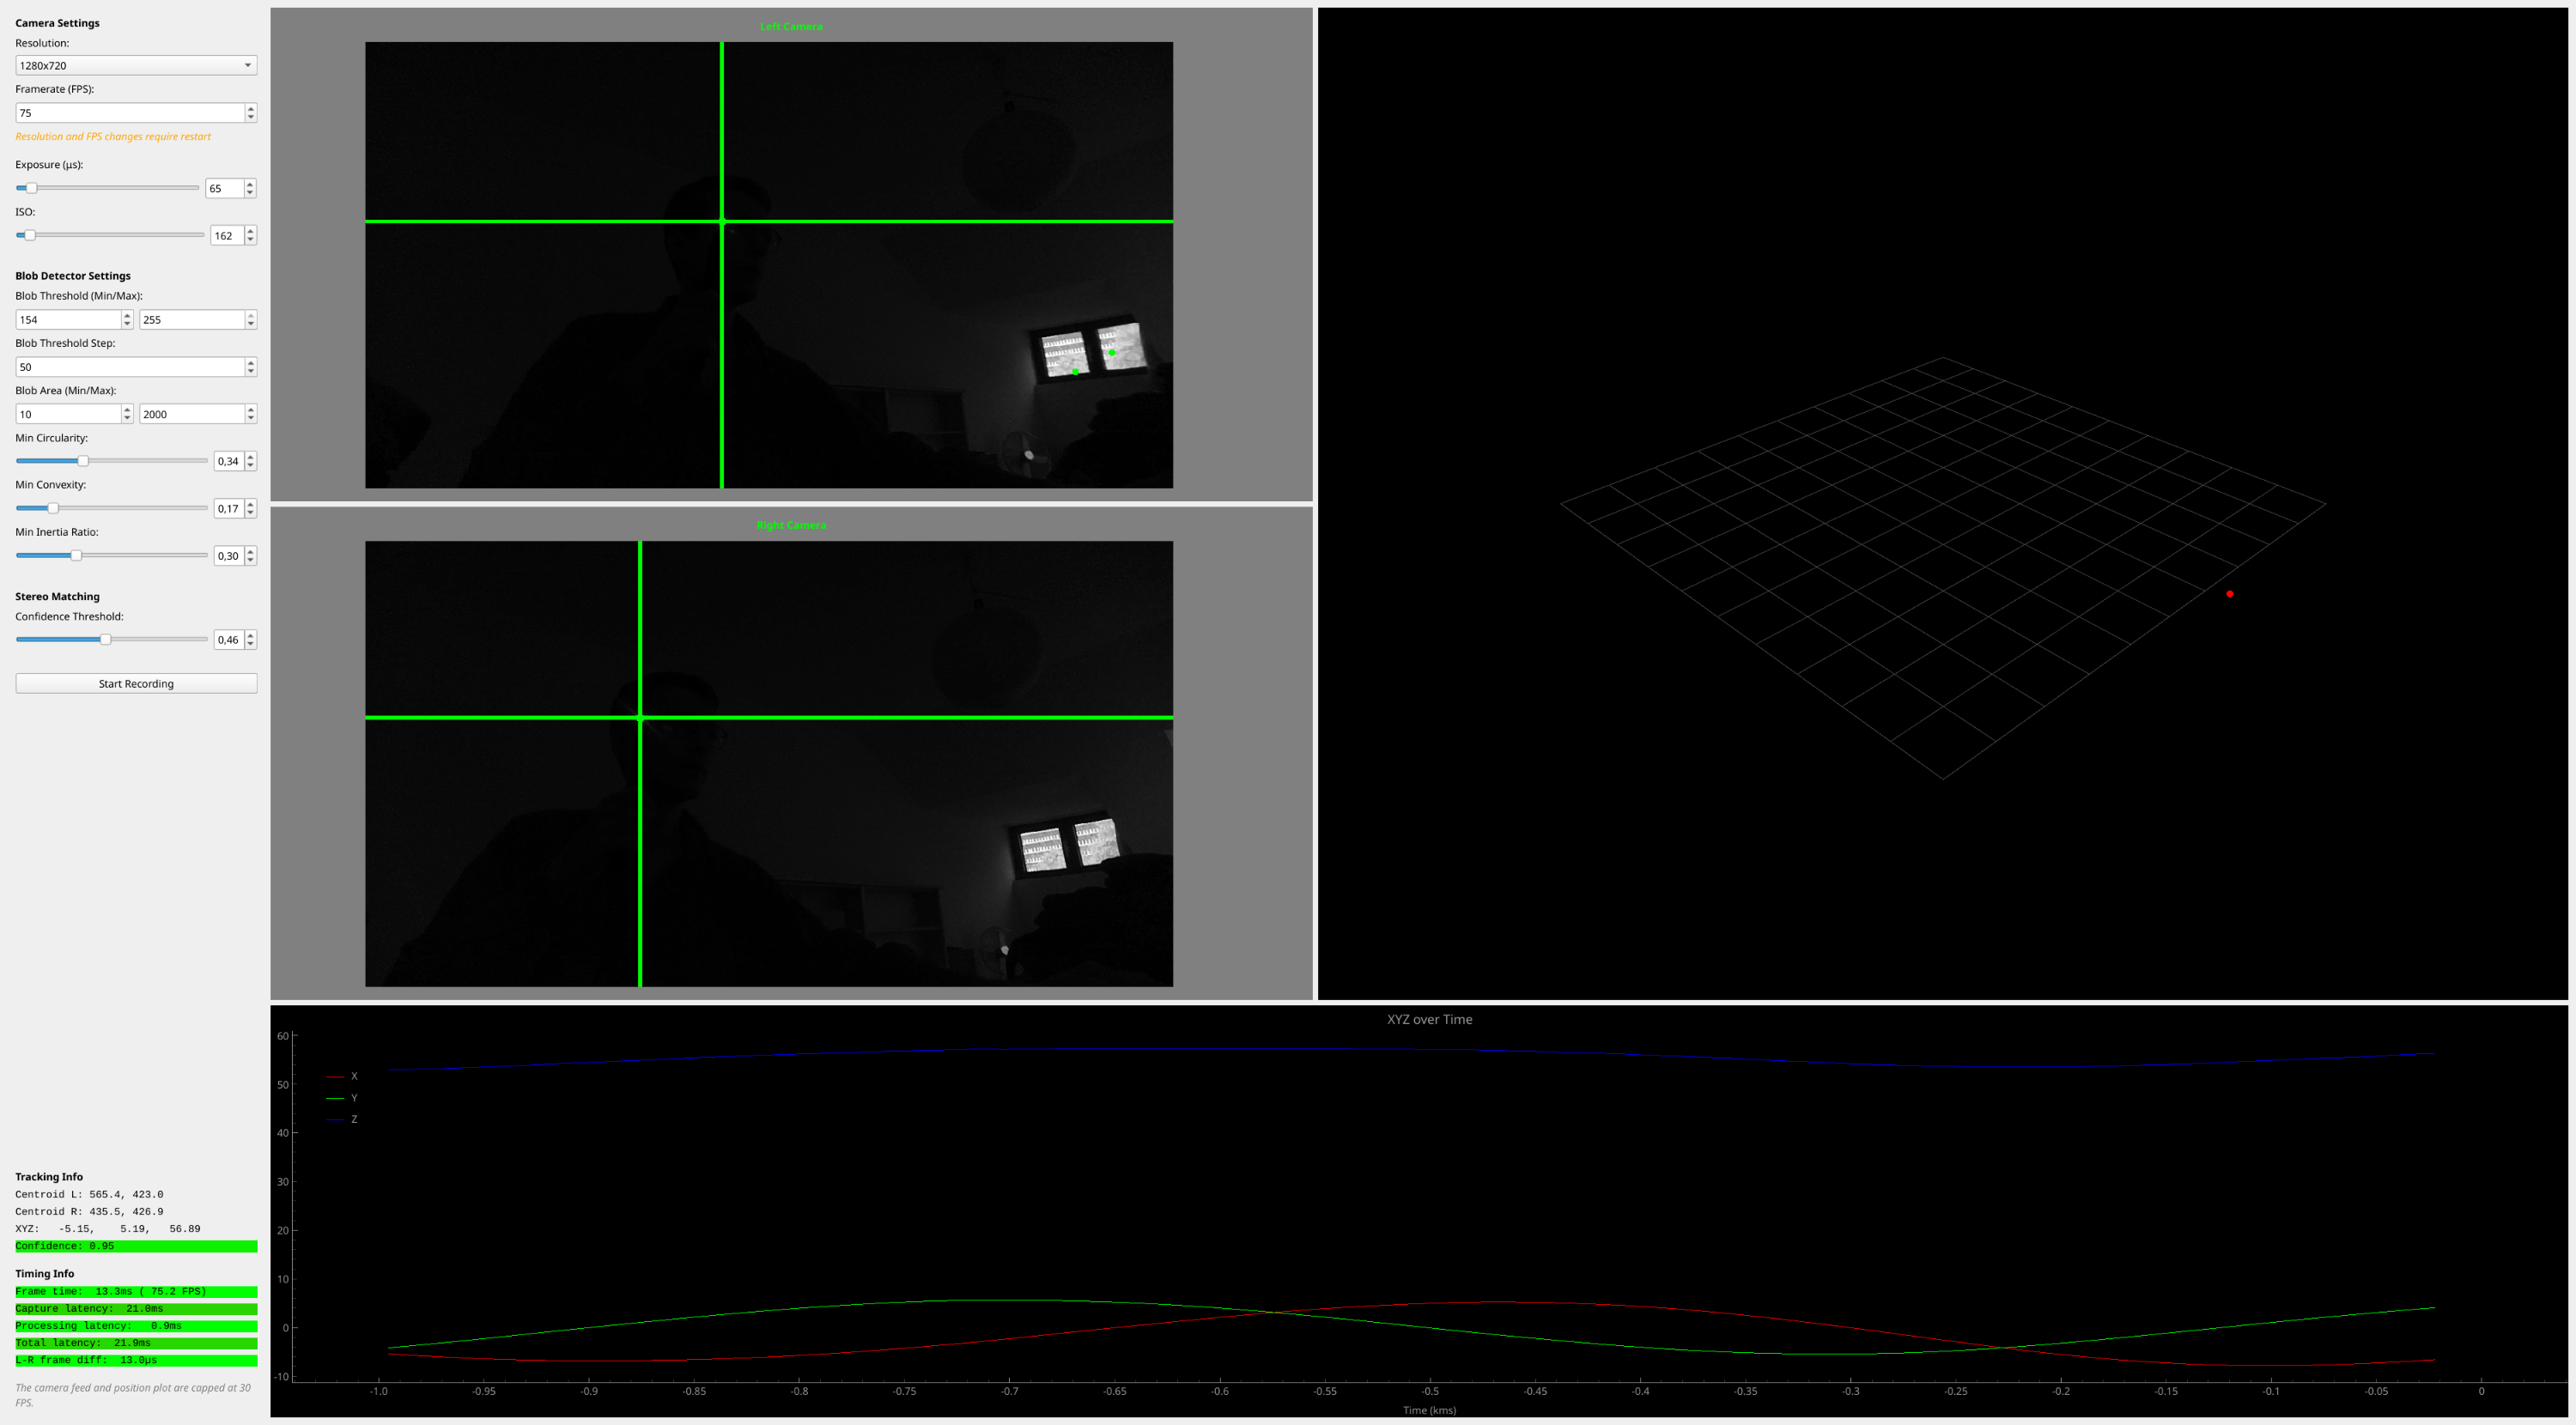
\includegraphics[width=\linewidth]{assets/point-tracker-ui.png}
  \caption{The user interface of the tracking software. Top left: settings; bottom left: status information. Left of center: the two camera images, each with a crosshair on the LED. Right: the 3D view. The red dot visualizes the computed coordinates. Bottom: a graph of the X (in red,), Y (in green), and Z coordinates (in blue) as a function of time.}
  \label{fig:tracker-ui}
\end{figure}

A major innovation is the user interface (\cref{fig:tracker-ui}). It shows both camera images, visualizes the detected coordinates as text, in 2D and 3D, both as curves and spatially, and displays several metrics on latency and processing speed.
These tools make it enormously easier to find optimal parameters for the blob detector and the camera and, if necessary, to adapt them to the ambient conditions and the performance of the computer used.
With the recording function, which is also new, the coordinates of the LED together with timestamps can be saved in CSV format for further processing and evaluation.

\section{Recording}
\label{sec:recording}

\begin{figure}[htbp]
  \centering
  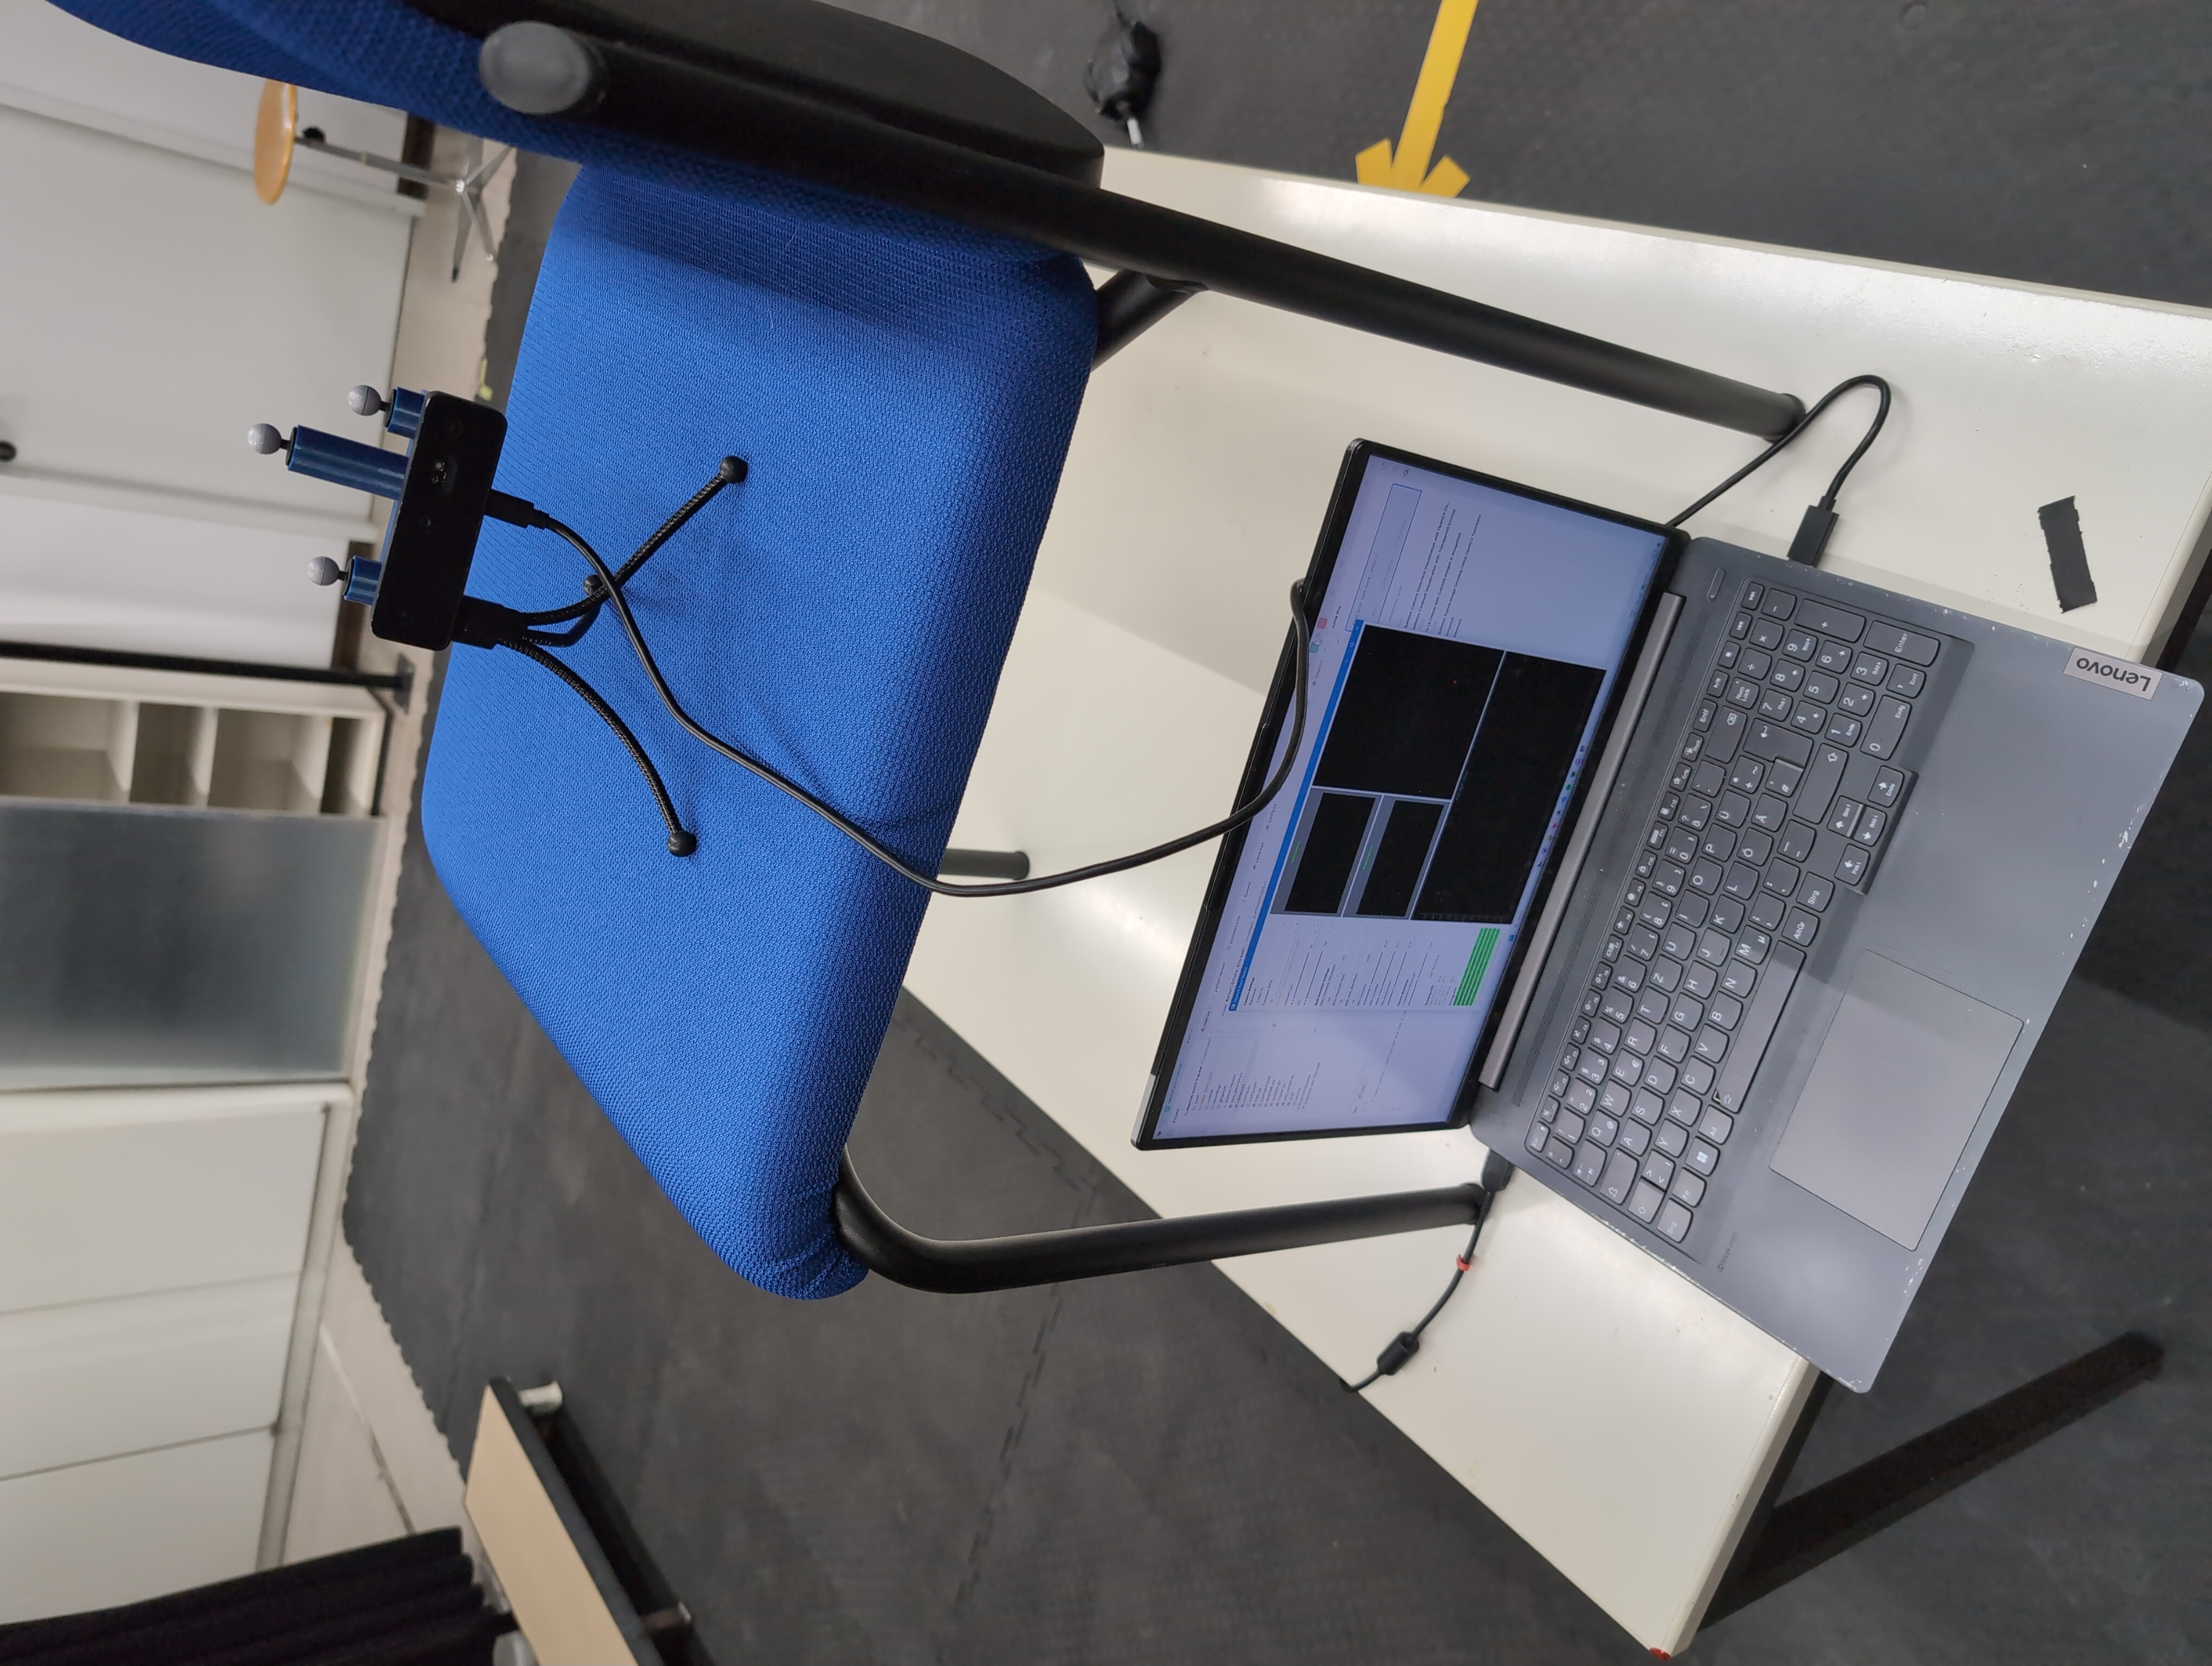
\includegraphics[width=0.6\linewidth]{assets/recording-setup.jpg}
  \caption{The stereo camera with tracking markers, connected to the recording software on my laptop in the motion capture studio}
  \label{fig:recording-setup}
\end{figure}

The signal processing is to be designed and tested on the basis of authentic motion capture data.
The recording takes place in the motion capture studio at Campus Deutz with the \emph{OAK-D} camera positioned inside the capture volume as shown in \cref{fig:recording-setup}.
For this purpose, the LED is attached to a pair of glasses together with a battery and a switch.
The test data therefore consists of head movements.
During the recordings, the LED moves within the area visible to the stereo camera at a distance of approx.\ 30~cm to 3~m.
To simulate different usage scenarios, there are four recordings for each of two different movement patterns:
On the one hand, slow movements with longer pauses, as would occur when using a screen, and on the other hand, fast, abrupt movements, as might occur in sports or dance.
The recordings last about 30 seconds each, except for one recording of slow movements that lasts two minutes.
All movements are recorded simultaneously using the \emph{OAK-D} at 75 Hz and using the \emph{OptiTrack} system at 120 Hz and exported to CSV-files.

\section{Temporal and Spatial Synchronization}
\label{sec:sync}

To process the recordings from the two different systems effectively, they must first be converted into a common data structure with aligned coordinate spaces and timestamps.
The point in time at which the LED first appears in the two recordings is used for temporal synchronization.
This works because the LED was manually switched on only once the two systems were already recording and the LED was visible to both.
A drawback is that possible differences in the latency of the two recordings are thereby compensated for, and this relevant (but not essential) information remains hidden due to the lack of a common clock.

Three tracking markers attached to the stereo camera allow the \emph{OptiTrack} cameras to capture their position and orientation relative to the LED.
They thus allow the LED coordinates to be mapped from the coordinate system of one camera system into that of the other by a combination of a translation and a rotation.
For this, each marker in the \emph{OAK-D} recording must be matched with the corresponding marker in the \emph{OptiTrack} recording.
The mount of the tracking markers is designed such that the markers form a triangle with three clearly different side lengths.
Each marker can therefore be identified by the length of the triangle side opposite to it, which does not depend on the order in which the markers are numbered.
Of the six possible assignments of the markers, the one for which these side lengths agree best is chosen.

Formally, let $s_i = \lVert \mathbf{p_j} - \mathbf{p_k} \rVert$ and $s'_i = \lVert \mathbf{p'_j} - \mathbf{p'_k} \rVert$ with $\{i, j, k\} = \{1, 2, 3\}$ denote the side lengths opposite to marker $i$.
With $S_3$ the set of all permutations of $\{1, 2, 3\}$, the assignment is
\[
  \sigma^* = \operatorname*{arg\,min}_{\sigma \in S_3} e(\sigma),
  \qquad
  e(\sigma) = \max_{i \in \{1, 2, 3\}} \lvert s_{\sigma(i)} - s'_i \rvert,
\]
so that the marker $\mathbf{p}_{\sigma^*(n)}$ corresponds to $\mathbf{p'_n}$.
The \emph{OptiTrack} markers are renumbered accordingly, so that in the following $\mathbf{p_n}$ refers to $\mathbf{p}_{\sigma^*(n)}$.

The rotation matrix $\mathbf{R}$ and the translation vector $\mathbf{t}$ map the positions of the three tracking markers $\mathbf{p_1}, \mathbf{p_2}, \mathbf{p_3}$ determined by the \emph{OptiTrack} system onto the positions of the tracking markers in the coordinate system of the stereo camera $\mathbf{p'_1}, \mathbf{p'_2}, \mathbf{p'_3}$, such that $\mathbf{p'_n} = \mathbf{R} \mathbf{p_n}+ \mathbf{t}$ holds for $n \in \{1, 2, 3\}$.
The coordinate system of the stereo camera has its origin at the optical center of the left camera lens, with the axes defined as x right, y up, and z forward from the point of view of the camera.
The tracking markers are rigidly attached to the camera, such that their positions can simply be measured once in the CAD model of the tracking marker mount and treated as constants.

Because the marker positions measured by the \emph{OptiTrack} system are subject to noise, the equation above can in general only be satisfied approximately.
$\mathbf{R}$ and $\mathbf{t}$ are therefore determined as the solution of the least squares problem
\[
  \min_{\mathbf{R}, \mathbf{t}} \sum_{n=1}^{3} \lVert \mathbf{R} \mathbf{p_n} + \mathbf{t} - \mathbf{p'_n} \rVert^2
  \quad \text{subject to} \quad \mathbf{R}^\top \mathbf{R} = \mathbf{I},
\]
which is solved with the algorithm of Kabsch \cite{kabsch1976, kabsch1978}.
First, both point sets are centered at their centroids $\bar{\mathbf{p}}$ and $\bar{\mathbf{p}}'$, which reduces the problem to finding $\mathbf{R}$; the translation then follows as $\mathbf{t} = \bar{\mathbf{p}}' - \mathbf{R} \bar{\mathbf{p}}$.
With the cross-covariance matrix of the centered point sets and its singular value decomposition
\[
  \mathbf{H} = \sum_{n=1}^{3} (\mathbf{p_n} - \bar{\mathbf{p}})(\mathbf{p'_n} - \bar{\mathbf{p}}')^\top = \mathbf{U} \mathbf{\Sigma} \mathbf{V}^\top,
\]
the optimal matrix is
\[
  \mathbf{R} = \mathbf{V} \mathbf{D} \mathbf{U}^\top,
  \qquad
  \mathbf{D} = \operatorname{diag}(1, 1, d).
\]
In the usual formulation, $d = \operatorname{sgn} \det(\mathbf{V} \mathbf{U}^\top)$ ensures $\det \mathbf{R} = +1$, so that $\mathbf{R}$ is a proper rotation \cite{kabsch1978}.
Here, however, the coordinate system of the stereo camera described above is left-handed, while that of the \emph{OptiTrack} system is right-handed.
No proper rotation can map one onto the other, so $d = -\operatorname{sgn} \det(\mathbf{V} \mathbf{U}^\top)$ is chosen instead, which yields $\det \mathbf{R} = -1$, i.e., $\mathbf{R}$ contains a reflection in addition to a rotation.
Without this adjustment, the tracked positions of the two systems are mirrored across the XY-plane.

\begin{figure}[htbp]
  \centering
  \begin{minipage}{0.49\linewidth}
    \centering
    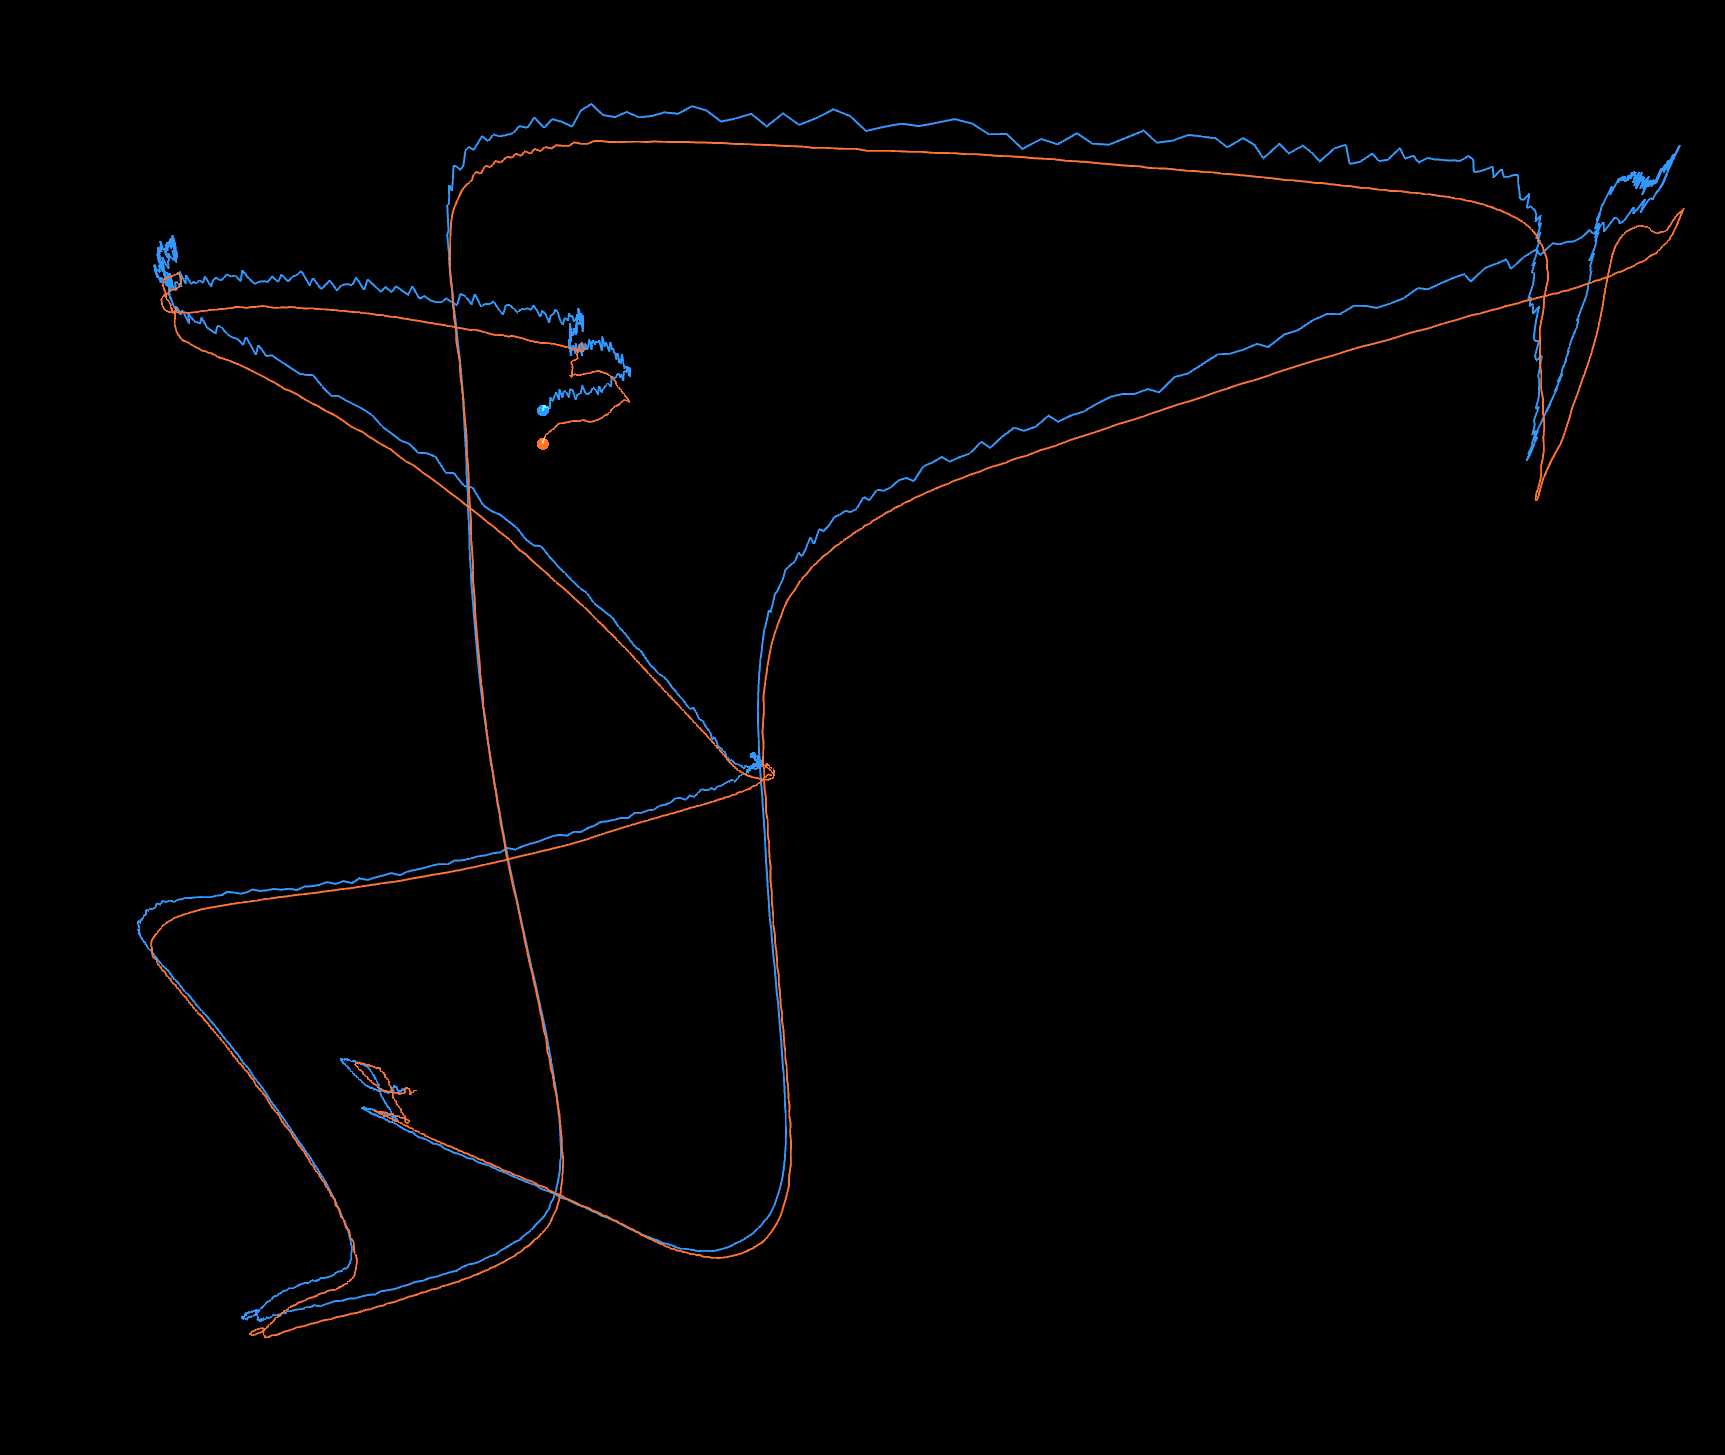
\includegraphics[width=\linewidth]{assets/aligned-tracks.png}
  \end{minipage}
  \hfill
  \begin{minipage}{0.49\linewidth}
    \centering
    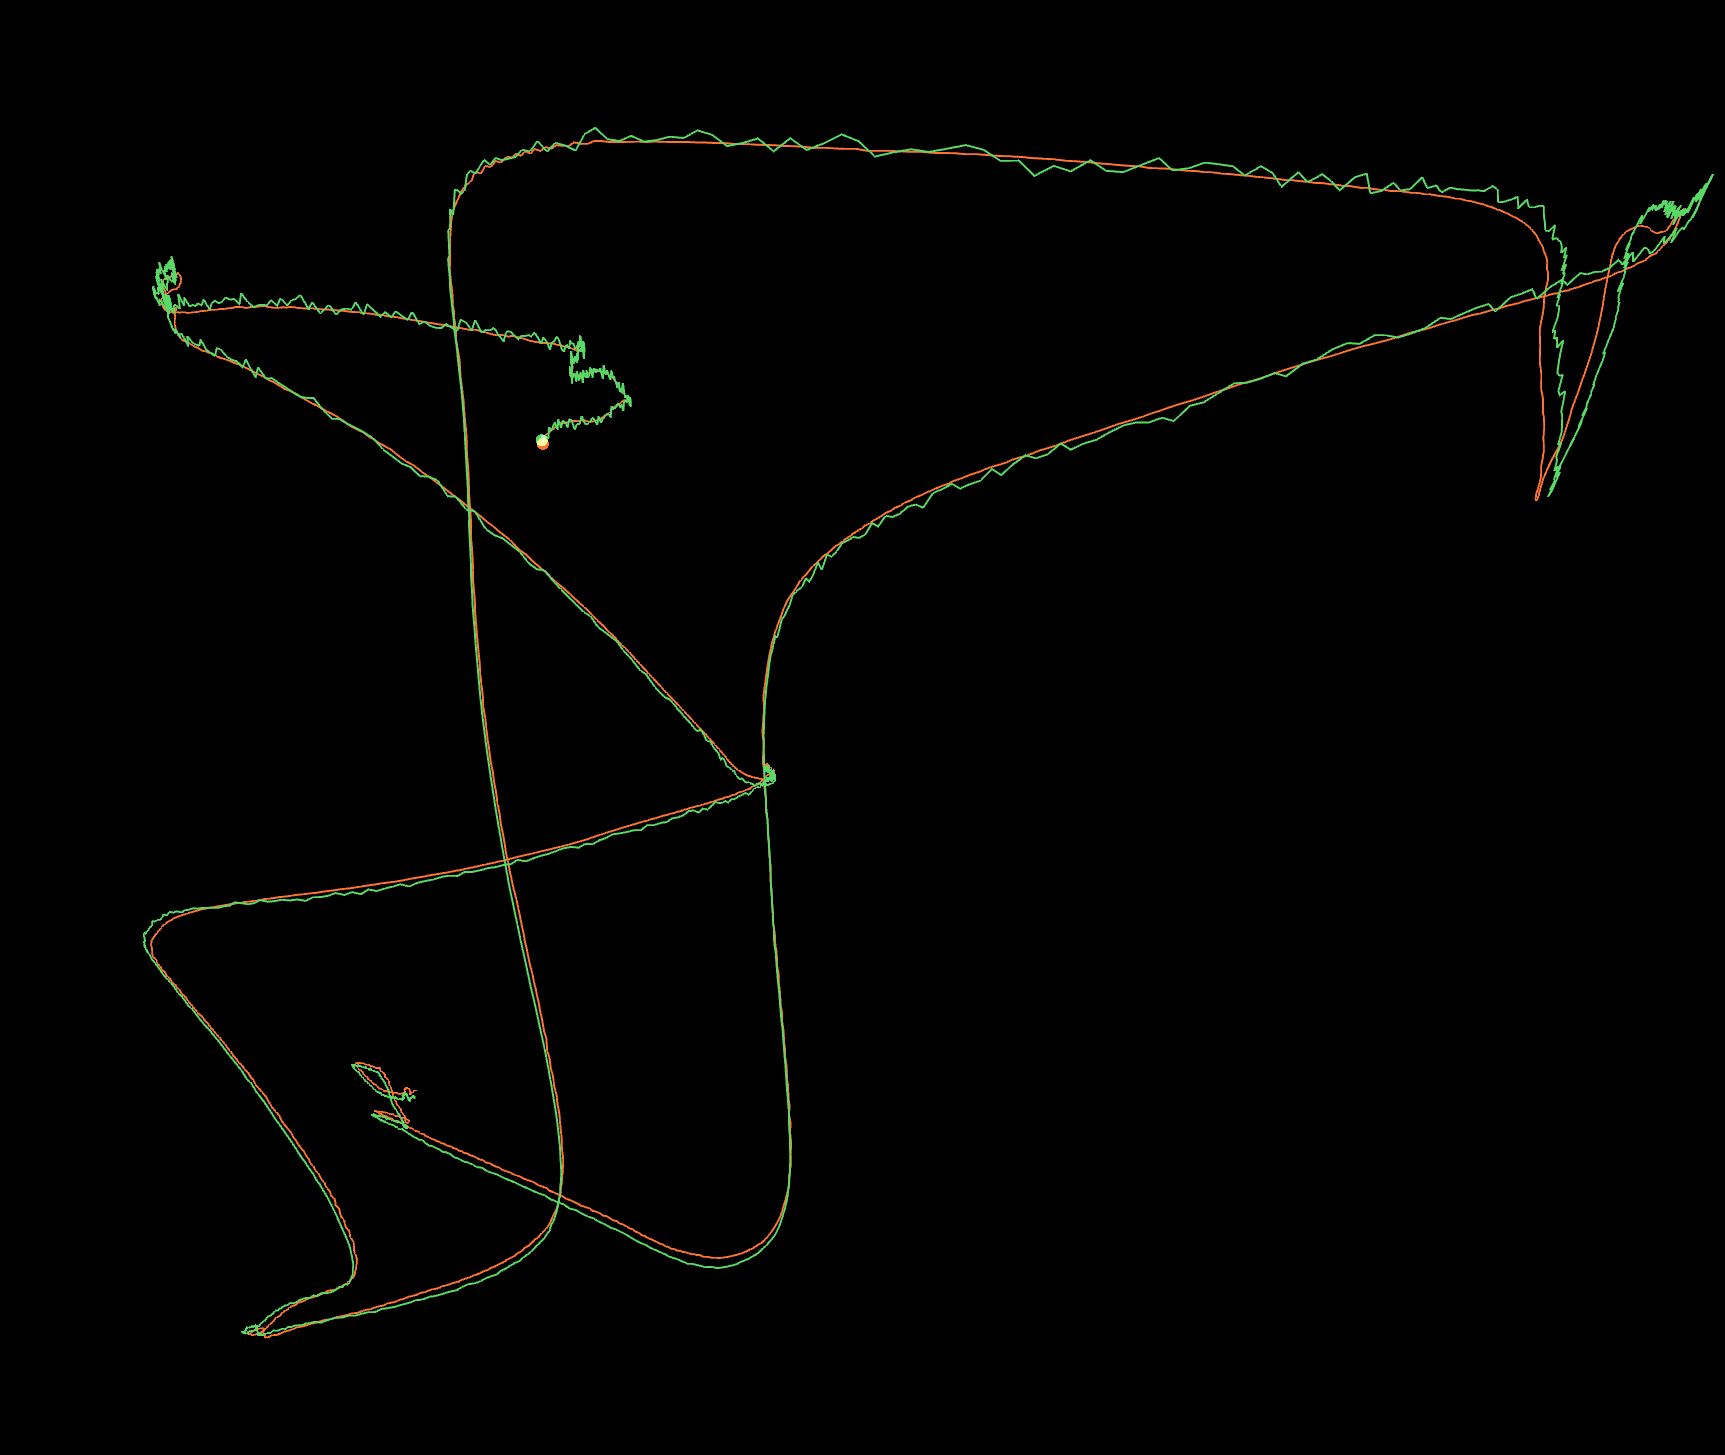
\includegraphics[width=\linewidth]{assets/aligned-fitted-tracks.png}
  \end{minipage}
  \caption{LED tracks recorded by the \emph{OAK-D} (blue, green) and the \emph{OptiTrack} system (orange). Left: coordinate spaces aligned using the camera marker coordinates; a nearly constant offset between the tracks remains. Right: coordinate spaces aligned using the LED coordinates.}
  \label{fig:aligned-tracks}
\end{figure}

To eliminate reference frame error (as seen in \cref{fig:aligned-tracks}), the LED coordinates may be used instead of the camera marker coordinates to align the coordinate spaces.
Instead of matching the static camera marker coordinates to each other, one of the tracks is resampled to the frequency of the other using linear intepolation, discarding any segments in which either system lost track of the LED.
The coordinates are then paired up, and the least squares problem as described above is solved on those pairs instead.
Although this technique is not practically applicable because it requires a ground truth, it is useful when evaluating filtering techniques since they cannot possibly compensate for this type of error anyway.

\section{Filtering}
\label{sec:filtering}

The triangulated coordinates are subject to noise, which is to be removed without distorting the actual motion.
Since the recordings are processed offline in this section, every sample may be used to estimate the position at any point in time, including samples captured later.

\subsection{Smoothing splines}

The track is split into segments at every point where the \emph{OAK-D} lost track of the LED, so that gaps are never bridged.
Each coordinate of a segment is filtered separately.
Let $t_1 < \dots < t_n$ denote the timestamps of a segment and $y_1, \dots, y_n$ the measured values of one coordinate.
The smoothing spline is the function $g$ with square-integrable second derivative that minimizes
\begin{equation}
  \label{eq:spline-objective}
  J_\lambda(g) = \sum_{j=1}^{n} \bigl(y_j - g(t_j)\bigr)^2 + \lambda \int_{t_1}^{t_n} g''(t)^2 \, dt,
  \qquad \lambda \geq 0.
\end{equation}
The first term measures how closely $g$ follows the samples, the second term measures its curvature, and the smoothing parameter $\lambda$ weighs the two against each other.
For $\lambda = 0$, $g$ interpolates the samples; for $\lambda \to \infty$, the curvature is forced to zero and $g$ becomes the least squares line through the samples.

\subsection{Generalized cross-validation}

The result depends strongly on $\lambda$, and a suitable value depends on the noise level and on the motion, both of which differ between recordings and between coordinates.
Instead of setting $\lambda$ by hand, it is chosen for each segment and coordinate by generalized cross-validation (GCV).
The implementation uses \texttt{make\_smoothing\_spline} from SciPy \cite{scipy2020}, which chooses $\lambda$ separately for each coordinate.
Segments with fewer than five samples are passed through unchanged.

\section{Prediction}
\label{sec:prediction}

The smoothing spline of \cref{sec:filtering} estimates the position at time $t$ from samples before and after $t$.
A display connected in real time has neither: when it renders a frame, only samples that the tracking software has already processed are available, and the frame is seen some time later.
The position must therefore be predicted.

\subsection{Real-time constraints}
\label{sec:real-time}

Sample $j$ is captured at $t_j$ but becomes available only at $a_j = t_j + \ell_j$, where the camera and processing latency $\ell_j$ is taken per sample from the detection timestamps in the \emph{OAK-D} recording.
A display requests a position at the instants $\tau_k = \tau_0 + k \Delta$, $\Delta = 1/75$~s, and needs the position at $\tau_k + h$, where $h$ is the latency still ahead (transport, rendering, and display).
To evaluate predictors under exactly these conditions, the recordings are replayed:
at each $\tau_k$, the predictor receives the samples with $a_j \leq \tau_k$ that it has not seen yet, is asked for the position at $\tau_k + h$, and the answer is stored with the timestamp $\tau_k + h$, so that it can be compared with the ground truth at the time it refers to.
A predictor never has access to later samples, which is also verified by a test ensuring that truncating a recording does not change any earlier output.
The simplest predictor, the \emph{zero-order hold}, returns the newest sample $y_{m(k)}$ and serves as the baseline.

\subsection{Windowed spline extrapolation}

The spline approach of \cref{sec:filtering} is adapted to real time by fitting a smoothing spline to the samples of a 300~ms trailing window which contains about 22 samples.
The smoothing parameter is fixed instead of being chosen by GCV\@.
On so few samples, individual samples entering and exiting the trailing window make GCV behave erratically.

\subsection{Constant-velocity Kalman filter}

The Kalman filter \cite{kalman1960} with a constant-velocity model \cite{barshalom2001} is used for comparison.
Its state for each coordinate is $\mathbf{x} = (p, v)^\top$.
Between two samples with interval $\delta_j = t_j - t_{j-1}$, the state evolves as
\[
  \mathbf{x}_j = \mathbf{F}_j \mathbf{x}_{j-1} + \mathbf{q}_j,
  \qquad
  \mathbf{F}_j = \begin{pmatrix} 1 & \delta_j \\ 0 & 1 \end{pmatrix},
  \qquad
  \mathbf{Q}_j = \operatorname{Cov}(\mathbf{q}_j) = \sigma_a^2 \begin{pmatrix} \delta_j^3/3 & \delta_j^2/2 \\ \delta_j^2/2 & \delta_j \end{pmatrix},
\]
which is the exact discretization of the white-noise acceleration model from \cref{sec:spline-interpretation}.
A sample measures the position, $y_j = \mathbf{H} \mathbf{x}_j + \varepsilon_j$ with $\mathbf{H} = (1 \;\, 0)$ and $\varepsilon_j \sim \mathcal{N}(0, \sigma_m^2)$.
For every arriving sample, the estimate $\hat{\mathbf{x}}$ and its covariance $\mathbf{P}$ are first propagated and then corrected with the measurement:
\begin{align*}
  \mathbf{x}^- &= \mathbf{F}_j \hat{\mathbf{x}}_{j-1}, &
  \mathbf{P}^- &= \mathbf{F}_j \mathbf{P}_{j-1} \mathbf{F}_j^\top + \mathbf{Q}_j, \\
  \mathbf{k} &= \frac{\mathbf{P}^- \mathbf{H}^\top}{\mathbf{H} \mathbf{P}^- \mathbf{H}^\top + \sigma_m^2}, &
  \hat{\mathbf{x}}_j &= \mathbf{x}^- + \mathbf{k} \, (y_j - \mathbf{H} \mathbf{x}^-), \qquad
  \mathbf{P}_j = (\mathbf{I} - \mathbf{k} \mathbf{H}) \mathbf{P}^-.
\end{align*}
The prediction for a requested frame is $\hat p + \hat v L_k$.
The filter starts with $\hat{\mathbf{x}}_1 = (y_1, 0)^\top$ and $\mathbf{P}_1 = \operatorname{diag}(\sigma_m^2, 10^6)$, i.e., with a practically unknown velocity.
Because $\mathbf{F}_j$, $\mathbf{Q}_j$, and $\sigma_m$ are the same for all coordinates, one covariance matrix serves all three.
The measurement noise is set to $\sigma_m = 0.1$~cm, while the process noise $\sigma_a$ determines the trade-off between noise and lag and is tuned in \cref{sec:evaluation}.

The Kalman filter is closely related to the smoothing spline.
Under the model above, the Kalman filter computes the expected state given all samples up to $t_j$, and the Rauch--Tung--Striebel smoother \cite{rauch1965} computes it given all samples of the segment.
By \cref{eq:lambda-noise}, the latter is exactly the smoothing spline with $\lambda = \sigma_m^2 / \sigma_a^2$ \cite{wahba1978, kohn1987}.
At the newest sample, the two coincide:
apart from the prior on the initial state, the Kalman estimate $(\hat p, \hat v)$ equals the value and slope at the end of a smoothing spline fitted to \emph{all} past samples.
The Kalman prediction is therefore the windowed spline extrapolation with $W \to \infty$ and without the cubic term of \cref{eq:spline-extrapolation}, and it inherits the velocity lag caused by the boundary.

This lag can be quantified.
For a constant sampling interval $\delta$ that is short compared with the time scale of the motion, the filter settles into a steady state that is well described by its continuous-time counterpart with process noise intensity $\sigma_a^2$ and measurement noise intensity $r = \sigma_m^2 \delta$.
Solving the algebraic Riccati equation yields the constant gains $k_p = \sqrt{2} \, \omega_0$ and $k_v = \omega_0^2$ with
\begin{equation}
  \label{eq:omega0}
  \omega_0 = \left( \frac{\sigma_a^2}{\sigma_m^2 \delta} \right)^{1/4} = (\lambda \delta)^{-1/4}.
\end{equation}
The estimation error thus obeys a second-order system with the characteristic polynomial $s^2 + \sqrt{2} \, \omega_0 s + \omega_0^2$, i.e., with natural frequency $\omega_0$ and damping $1/\sqrt{2}$.
By \cref{eq:lambda-noise}, $\omega_0$ equals $2 \pi f_c$ of the smoothing spline in \cref{eq:transfer}, so the causal filter and the offline smoother operate on the same time scale.
If the target moves with constant acceleration $a$, the estimation error $(e_p, e_v)$ satisfies $\dot e_p = e_v - k_p e_p$ and $\dot e_v = a - k_v e_p$ and settles at $e_p = a / \omega_0^2$ and $e_v = \sqrt{2} \, a / \omega_0$.
Inserted into \cref{eq:prediction-error}, the prediction error becomes
\begin{equation}
  \label{eq:kalman-lag}
  e(L) = \frac{a}{\omega_0^2} + \frac{\sqrt{2} \, a}{\omega_0} L + \frac{a}{2} L^2 = \frac{a}{2} \left( L + \frac{\sqrt{2}}{\omega_0} \right)^2.
\end{equation}
The filter behaves as if the lead were extended by $\sqrt{2} / \omega_0$.
A larger $\sigma_a$ shortens this delay in proportion to $\sigma_a^{-1/2}$, but the steady-state standard deviation of $\hat v$, $(\sqrt{2} \, r^{1/4} \sigma_a^{3/2})^{1/2}$, grows in proportion to $\sigma_a^{3/4}$, and it is multiplied by $L$ in the prediction.
In practice, the two methods differ in the following respects:
\begin{itemize}
  \item \emph{Memory.} The Kalman filter weighs past samples with an exponentially decaying weight whose time constant follows from $\sigma_a / \sigma_m$; the window discards everything older than $W$, which increases the variance of $\hat v$ if $W$ is shorter than that time constant.
  \item \emph{Cost.} The Kalman filter needs a constant number of operations per sample, whereas the spline is fitted anew from all samples of the window for every frame.
  \item \emph{Parameters.} $\sigma_m$ and $\sigma_a$ are physical quantities that can be estimated from recordings, and irregular sampling intervals (e.g., dropped frames) enter the model directly through $\delta_j$.
\end{itemize}

\section{Evaluation}
\label{sec:evaluation}

\subsection{Setup and metrics}

The evaluation uses the four recordings of slow movements (\emph{slow2}--\emph{slow5}) and three of the four recordings of fast movements (\emph{fast2}--\emph{fast4}).
The recording \emph{fast1} is excluded because its two tracks cannot be aligned.
The two versions contain completely different movements due to user error during recording.
All \emph{OAK-D} tracks are mapped into the \emph{OptiTrack} frame with the transform fitted to the LED coordinates as described in \cref{sec:sync}, so that the remaining deviations are those a filter could in principle affect.
Movement speeds (from the \emph{OptiTrack} tracks) have a median of about 5--8~cm/s and a 95th percentile of 35--49~cm/s for the slow recordings, and a median of 95--121~cm/s and a 95th percentile of 190--206~cm/s for the fast recordings.
All scripts and generated tables are part of the project repository.

Accuracy is measured by the Euclidean distance $e_k = \lVert \hat{\mathbf{y}}_k - \mathbf{y}^*(s_k) \rVert$ between an estimate $\hat{\mathbf{y}}_k$ for time $s_k$ and the \emph{OptiTrack} position $\mathbf{y}^*$ at that time, linearly interpolated between the 120~Hz samples.
Estimates falling into gaps of the ground truth are excluded.
Reported are the root mean square error $\mathrm{RMSE} = (\frac{1}{K} \sum_k e_k^2)^{1/2}$ and the 95th and 99th percentiles P95 and P99 of $e_k$, all in centimeters.
The RMSE is dominated by large deviations, whereas the percentiles show how often a given deviation is exceeded.

For a display, it also matters how calm the estimate is: a predictor that jitters around the correct position may achieve a small RMSE yet produce a shaking image.
Two smoothness measures are therefore computed on the uniformly sampled output of the predictors in \cref{sec:prediction}.
The \emph{jerk ratio} is the RMS of the third difference quotient $(\hat{\mathbf{y}}_{k+3} - 3 \hat{\mathbf{y}}_{k+2} + 3 \hat{\mathbf{y}}_{k+1} - \hat{\mathbf{y}}_k) / \Delta^3$ divided by the same quantity computed for the ground truth on the same time grid.
The \emph{step ratio} is the 99th percentile of the frame-to-frame movement $\lVert \hat{\mathbf{y}}_{k+1} - \hat{\mathbf{y}}_k \rVert$, again relative to the ground truth.
A ratio of 1 means that the output moves exactly as much as the real motion; values above 1 indicate added jitter.

\subsection{Offline filtering}

\begin{table}[htbp]
  \centering
  \caption{Deviation from the ground truth before and after smoothing with the GCV spline (raw / GCV) in cm, the standard deviation of the raw deviation per axis, and the RMS $\hat\sigma$ of the component removed by the spline.}
  \label{tab:filtering}
  \small
  \begin{tabular}{lccccc}
\hline
Rec. & RMSE & P95 & P99 & Std.\ $x$ / $y$ / $z$ (raw) & $\hat\sigma$ \\
\hline
slow2 & 0.64 / 0.62 & 1.26 / 1.26 & 1.55 / 1.45 & 0.35 / 0.29 / 0.45 & 0.126 \\
slow3 & 0.46 / 0.46 & 0.95 / 0.95 & 1.20 / 1.12 & 0.23 / 0.15 / 0.37 & 0.072 \\
slow4 & 0.47 / 0.44 & 0.80 / 0.78 & 0.96 / 0.91 & 0.28 / 0.15 / 0.34 & 0.147 \\
slow5 & 0.85 / 0.81 & 1.72 / 1.74 & 2.57 / 2.30 & 0.41 / 0.34 / 0.67 & 0.244 \\
\hline
fast2 & 0.64 / 0.64 & 1.07 / 1.06 & 1.43 / 1.36 & 0.45 / 0.23 / 0.40 & 0.098 \\
fast3 & 0.53 / 0.51 & 1.01 / 0.96 & 1.47 / 1.31 & 0.25 / 0.19 / 0.43 & 0.151 \\
fast4 & 1.86 / 0.67 & 0.84 / 0.96 & 1.46 / 2.65 & 0.58 / 0.60 / 1.66 & 1.699 \\
\hline
\end{tabular}

\end{table}

\begin{figure}[htbp]
  \centering
  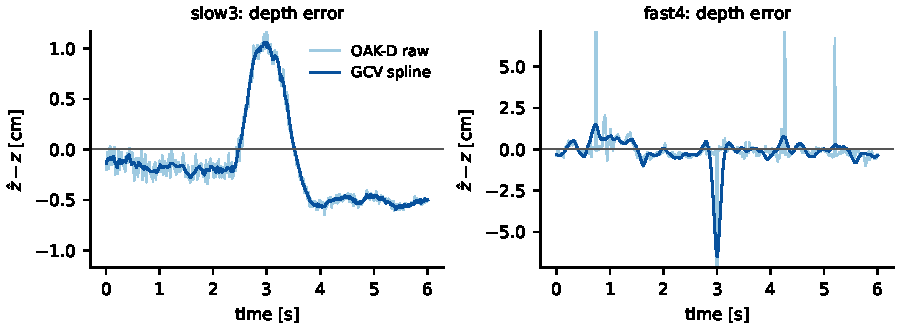
\includegraphics[width=\linewidth]{assets/filtering-excerpt.pdf}
  \caption{Deviation of the depth coordinate from the ground truth before and after smoothing. Left: a typical slow recording, where the deviation varies slowly and passes through the spline. Right: \emph{fast4} with isolated outliers, which the spline flattens but spreads out in time.}
  \label{fig:filtering-excerpt}
\end{figure}

\Cref{tab:filtering} shows that the GCV spline improves the accuracy only marginally.
On six of the seven recordings, the RMSE decreases by at most 6\%, from 0.85 to 0.81~cm in the best case.
The component removed by the spline has an RMS of only $\hat\sigma = 0.07$--$0.24$~cm, while the deviations are 0.46--0.85~cm.

The reason becomes apparent when the deviation is split into a component $\mathbf{e}_{\text{low}}$ below and a component $\mathbf{e}_{\text{high}}$ above the cutoff frequency $f_c$ of \cref{eq:transfer}.
The spline removes $\mathbf{e}_{\text{high}}$ and preserves $\mathbf{e}_{\text{low}}$, and since the two components are orthogonal, the RMSE after smoothing is approximately $(\mathrm{RMSE}^2 - \hat\sigma^2)^{1/2}$.
For \emph{slow5}, this yields $(0.852^2 - 0.244^2)^{1/2} = 0.816$~cm compared with the measured 0.810~cm.
On these six recordings, the cutoff frequencies resulting from the GCV-chosen $\lambda$ lie between 4 and 11~Hz, and a spectral analysis of the raw deviations shows that 81--99\% of their power lies below the cutoff of the respective axis.
The deviation of the \emph{OAK-D} is thus not predominantly white noise, but a slowly varying error that no low-pass filter can separate from the motion.
A residual time offset between the two systems, which would produce an error proportional to the velocity, can be ruled out:
shifting the \emph{OAK-D} tracks by up to $\pm 80$~ms reduces the RMSE by at most 0.01~cm.
The error is therefore spatial, as the left plot of \cref{fig:filtering-excerpt} illustrates, where the depth error rises by about 1~cm while the LED passes through part of the volume and then settles at a different level.
This is consistent with the geometry of stereo triangulation: with focal length $f$ and baseline $B$, the depth $z = fB/d$ follows from the disparity $d$, so a small disparity error $\delta d$ caused by imperfect calibration or rectification produces a depth error
\[
  \delta z \approx \frac{z^2}{fB} \, \delta d
\]
that changes smoothly with the position of the LED.
Accordingly, in most recordings the depth axis has the largest standard deviation, and GCV chooses a smaller cutoff for it than for the lateral axes.
Such an error is indistinguishable from motion for any filter that sees only the \emph{OAK-D} data.

\emph{fast4} is the exception.
Isolated outliers of up to 6~cm (right plot of \cref{fig:filtering-excerpt}), presumably incorrect detections, dominate its RMSE, which the spline reduces from 1.86 to 0.67~cm.
At the same time, however, P95 and P99 increase from 0.84 to 0.96~cm and from 1.46 to 2.65~cm.
The spline does not remove an outlier but distributes it over the width of its kernel:
the squared error of a single large deviation is replaced by many small ones, which lowers the RMSE but pushes more samples above the percentiles.
Moreover, the outliers inflate the apparent noise level, so GCV selects cutoff frequencies of only 3--5~Hz for this recording and smooths the actual motion more strongly than necessary.
A robust rejection of outliers before smoothing would be the better remedy here.

\subsection{Prediction}

The measurement noise of the Kalman filter is fixed at $\sigma_m = 0.1$~cm, the order of magnitude of the component $\hat\sigma$ removed by the offline spline (0.07--0.24~cm on the recordings without outliers, \cref{tab:filtering}).
The process noise $\sigma_a$ and the smoothing parameter $\lambda$ of the windowed spline ($W = 300$~ms) are each tuned once for all seven recordings at $h = 50$~ms.
Since the image should above all be calm, the tuning minimizes the jerk ratio $\rho_i$ of recording $i$, while an RMSE above that of the zero-order hold is penalized:
\[
  \min \; \max_i \left( \lvert \ln \rho_i \rvert + 100 \max\!\left(0, \frac{\mathrm{RMSE}_i}{\mathrm{RMSE}_i^{\text{hold}}} - 1\right) \right).
\]
The maximum over the recordings prevents the slow recordings, which are in the majority, from determining the parameter alone.
The search runs on a logarithmic grid followed by a bounded scalar minimization and yields $\sigma_a = 6.37~\text{cm/s}^{3/2}$ and $\lambda = 1.61 \cdot 10^{-4}~\text{s}^3$.
Although the two parameters were tuned independently, they agree well with \cref{eq:lambda-noise}, which predicts $\lambda = \sigma_m^2 / \sigma_a^2 = 2.46 \cdot 10^{-4}~\text{s}^3$; the corresponding natural frequencies \cref{eq:omega0} are $\omega_0 = 23.5$ and $26.1$~rad/s.
The median lead \cref{eq:lead} at $h = 0$ is $L = 31$~ms, consisting of the median camera latency of 25~ms and the time until the next display frame.

\begin{table}[htbp]
  \centering
  \caption{Prediction accuracy (in cm) and smoothness, averaged over the recordings of each movement pattern, for three horizons $h$ added to the measured camera latency.}
  \label{tab:prediction}
  \small
  \begin{tabular}{lllcccc}
\hline
Regime & $h$ [ms] & Predictor & RMSE & P95 & Jerk ratio & Step ratio \\
\hline
slow & 0 & Hold & 0.84 & 1.62 & 9.0 & 1.53 \\
 &  & Spline refit & 0.65 & 1.24 & 3.3 & 1.11 \\
 & 50 & Hold & 1.61 & 3.48 & 9.1 & 1.52 \\
 &  & Spline refit & 0.81 & 1.52 & 3.9 & 1.23 \\
 & 100 & Hold & 2.47 & 5.54 & 8.9 & 1.53 \\
 &  & Spline refit & 1.15 & 2.24 & 9.6 & 1.74 \\
\hline
fast & 0 & Hold & 4.24 & 6.84 & 40.5 & 2.18 \\
 &  & Spline refit & 3.45 & 5.75 & 22.3 & 1.56 \\
 & 50 & Hold & 9.98 & 16.21 & 41.1 & 2.18 \\
 &  & Spline refit & 8.46 & 14.85 & 33.2 & 2.36 \\
 & 100 & Hold & 15.50 & 25.11 & 41.8 & 2.19 \\
 &  & Spline refit & 16.09 & 27.92 & 61.7 & 3.76 \\
\hline
\end{tabular}

\end{table}

\begin{figure}[htbp]
  \centering
  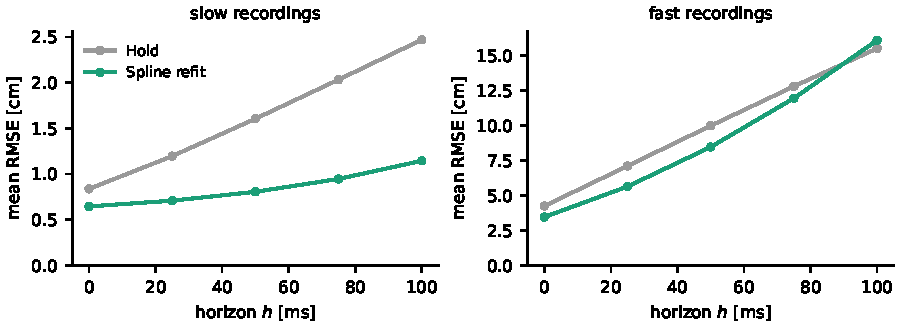
\includegraphics[width=\linewidth]{assets/prediction-horizon.pdf}
  \caption{Mean RMSE of the predictors as a function of the horizon $h$.}
  \label{fig:prediction-horizon}
\end{figure}

\begin{figure}[htbp]
  \centering
  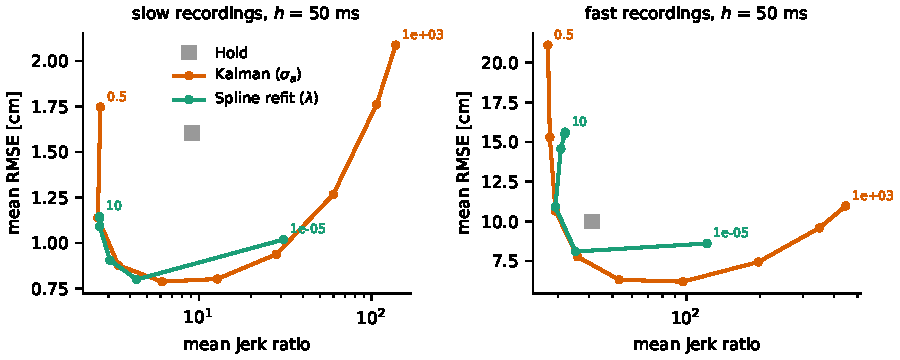
\includegraphics[width=\linewidth]{assets/prediction-sweep.pdf}
  \caption{Trade-off between accuracy and smoothness at $h = 50$~ms when varying $\sigma_a$ of the Kalman filter ($0.5$ to $1000$) and $\lambda$ of the windowed spline ($10^{-5}$ to $10$). The labels mark the ends of each sweep.}
  \label{fig:prediction-sweep}
\end{figure}

\begin{figure}[htbp]
  \centering
  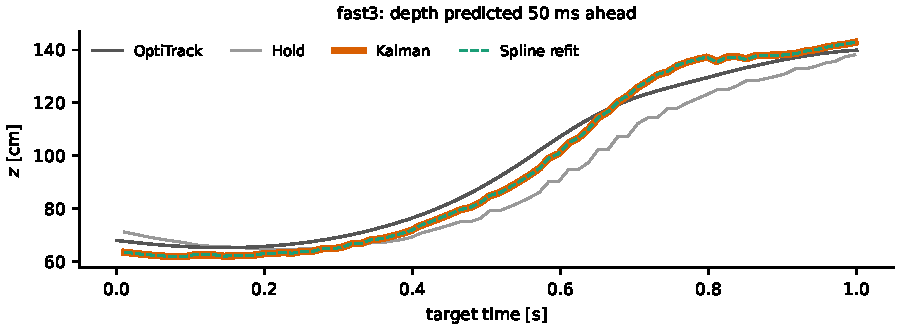
\includegraphics[width=\linewidth]{assets/prediction-excerpt.pdf}
  \caption{Depth predicted 50~ms ahead during a fast movement. The hold lags behind by the entire lead and shows steps; both predictors lag during the acceleration and overshoot when the movement stops. The Kalman filter (wide line) and the windowed spline (dashed) nearly coincide.}
  \label{fig:prediction-excerpt}
\end{figure}

\paragraph{Slow movements}
\Cref{tab:prediction} and \cref{fig:prediction-horizon} show that both predictors clearly improve on the zero-order hold for slow movements.
The RMSE decreases by 23\% without an additional horizon (0.84 to 0.65~cm), by 50\% at $h = 50$~ms (1.61 to 0.80~cm), and by 57\% at $h = 100$~ms (2.47 to 1.07~cm).
At $h = 50$~ms, the prediction is thus more accurate than the hold without any additional latency.
At $h = 0$, the RMSE of 0.65~cm hardly exceeds the mean offline deviation of the raw data of 0.60~cm (\cref{tab:filtering}):
the remaining error is essentially the systematic triangulation error discussed above, which no predictor can remove.
The output of both predictors is also three times calmer than that of the hold (jerk ratio 3.1 versus 9.0 at $h = 0$).
The high jerk ratio of the hold does not depend on $h$ and is caused by its steps:
since the display frames are not synchronized with the camera frames and the latency varies, some display frames repeat a sample while the next one skips a sample.

The error of the hold follows the approximation $\mathbf{v} L$ from \cref{sec:real-time}.
With the RMS speed of the slow recordings of 17.9~cm/s, the median lead $L = h + 31$~ms, and the error floor $b = 0.60$~cm combined in quadrature, $(b^2 + v_{\text{rms}}^2 L^2)^{1/2}$ predicts 0.82, 1.57, and 2.42~cm for the three horizons, compared with the measured 0.84, 1.61, and 2.47~cm.
With the tuned $\sigma_a$, the delay in \cref{eq:kalman-lag} is $\sqrt{2} / \omega_0 = 60$~ms.
Since the accelerations of slow movements are small, the quadratic error remains of the order of the error floor, which explains why prediction almost halves the error here.

\paragraph{Fast movements}
For fast movements, the benefit is small.
The Kalman filter reduces the RMSE by 11\% at $h = 0$, by 15\% at $h = 50$~ms (9.98 to 8.51~cm), and by only 5\% at $h = 100$~ms, where the windowed spline is even worse than the hold (16.09 versus 15.50~cm).
The hold approximation again matches: with an RMS speed of 121.8~cm/s, $v_{\text{rms}} L$ predicts 3.8, 9.9, and 16.0~cm, compared with the measured 4.24, 9.98, and 15.50~cm.
For the predictors, \cref{eq:kalman-lag} with the RMS acceleration of 1022~cm/s$^2$ gives 4.2, 10.2, and 18.6~cm, compared with the measured 3.77, 8.51, and 14.77~cm.
The approximation overestimates the error because it assumes a constant acceleration, whereas the acceleration of a head movement changes its sign within a fraction of a second.
Nevertheless, it explains the essential effect:
the filter's own delay of 60~ms is more than twice the camera latency, so the extrapolation effectively bridges 90 to 190~ms, and over such leads the unmodelled acceleration dominates.
\Cref{fig:prediction-excerpt} shows the result: the predictions lag during the acceleration and overshoot by several centimeters when the movement stops.

The sweep in \cref{fig:prediction-sweep} shows that this is a consequence of the tuning rather than of the method.
With $\sigma_a = 57.8$, the delay shrinks to 20~ms and the RMSE of the fast recordings drops to 6.2~cm, 38\% below the hold, but their jerk ratio rises from 33 to 97, and the slow recordings become markedly less calm (jerk ratio 28 instead of 5).
This is the conflict from \cref{eq:kalman-lag}: shortening the delay requires a larger $\sigma_a$, which amplifies the noise in $\hat v$.
No single parameter serves both movement patterns.
For the windowed spline, large values of $\lambda$ turn the fit into a least squares line over the whole window, whose velocity refers to the middle of the window and thus lags by $W/2 = 150$~ms, while very small values make the output unstable (jerk ratio 31 and 121 at $\lambda = 10^{-5}$).

The windowed spline and the Kalman filter perform almost identically up to $h = 50$~ms, as expected from their equivalence.
Only at $h = 100$~ms does the spline fall behind (16.09 versus 14.77~cm, jerk ratio 61.7 versus 45.0), which is consistent with the cubic term of \cref{eq:spline-extrapolation}, whose contribution grows with $L^3$.

\subsection{Conclusion}

The offline smoothing with GCV splines works as intended, in that it adapts the smoothing parameter automatically to each recording and axis.
It is nevertheless of little use for the accuracy of the \emph{OAK-D} tracking, since it reduces the RMSE by at most 6\%.
The dominant error is a slowly varying, position-dependent triangulation error with an RMSE of 0.46 to 0.85~cm, which lies in the passband of every filter that preserves the motion.
It has to be reduced by better calibration, not by filtering.
Outliers, on the other hand, are only spread out by the spline and should be rejected beforehand.

For slow movements, as they occur in front of a screen, real-time prediction is effective:
it halves the error at horizons of 50 to 100~ms and brings it close to the error floor.
For fast movements, neither predictor is effective, with an RMSE of 8.5~cm at $h = 50$~ms and an improvement of at most 15\% over not predicting at all.
Even in the best case, the accuracy remains far from the few millimeters required by the parallax barrier display of \cref{sec:background}.

The windowed spline extrapolation offers no advantage over the Kalman filter.
Both are the same estimator, differing only in the finite window and the cubic extrapolation term, which degrades the spline at long leads; in addition, the spline has to be refitted for every frame.
Since the prediction error grows quadratically with the effective lead, the most promising improvements are reducing the latency of the tracking system itself and adapting the process noise to the movement, for example by switching between several motion models \cite{barshalom2001}.

\bibliographystyle{siamplain}
\bibliography{references}

\end{document}
